\section{Lecture 4: Mining Diverse Patterns}

\subsection{Mining Multi- Level Associations}

Items often form hierarchies. How to set min-support thresholds? \textbf{Level-reduced min-support}: items at the lower level are expected to have lower support.\\

Efficient mining: \textbf{shared} multi-level mining. Use the lowest min-support to pass down the set of candidates.\\

Redundancy\footnote{Redundancy - избыточность} filtering: some rules may be redundant due to <<ancestor>>\footnote{Ancestor -- предок} relationships between items. A rule is \textbf{redundant} if:
\begin{itemize}
\item its support is close to the <<expected>> value, according to its <<ancestor>> rule
\item it has a similar confidence as its <<ancestor>>.
\end{itemize}\\

It is necessary to have customized min-support settings for different kinds of items: group-based <<individualized>> min-support.

%--
\subsection{Mining Multi-Dimensional Associations}
Rules can be single-dimensional or multi-dimensional:
\begin{itemize}
\item Single-dimentional: 
\begin{equation*}
\mathrm{buys}(X, \text{<<milk>>}) \Rightarrow \mathrm{buys}(X, \text{<<bread>>})
\end{equation*}
\item Inter-dimension association rule: 
\begin{equation*}
\mathrm{age}(X, \text{<<18-25>>}) \wedge \mathrm{occupation}(X, \text{<<student>>}) \Rightarrow \mathrm{buys}(X, \text{<<coke>>})
\end{equation*}
\item Hybrid-dimension association rules: 
\begin{equation*}
\mathrm{age}(X, \text{<<18-25>>}) \wedge \mathrm{buys}(X, \text{<<popcorn>>}) \Rightarrow \mathrm{buys}(X, \text{<<coke>>})
\end{equation*}
\end{itemize}


Attributes can be categorical or numerical

%--    
\subsection{Mining Quantitative Associations}

Methods:
\begin{itemize}
\item Static discretization based on predefined concept hierarchies
\item Dynamic discretization based on data distribution
\item Clustering: distance-based association
\item Deviation analysis
\end{itemize}

%--
\subsection{Mining Negative Correlations}
\begin{itemize}
\item Rare patterns = very low support but interesting
\item Negative patterns = negatively correlated, unlikely to happen together
\end{itemize}

A support-based definition: if itemsets A and B are both frequent but rarely occur together, i.e., $\sup(A \cup B) << \sup (A) \times \sup(B)$ then A and B are negatively correlated.\\

The support-based definition is not null-invariant!\\

A Kulczynski measure-based definition: if itemsets A and B are frequent but $\frac{P(A \mid B) + P(B \mid A)}{2} < \varepsilon$, where $\varepsilon$ is a negative pattern threshold, then A and B are negatively correlated.

%--
\subsection{Mining Compressed Patterns}
\subsubsection{Mining Compressed Patterns}
Pattern distance measure:
\begin{equation*}
Dist(P_1, P_2)=1-\frac{\abs{T(P_1) \cap T(P_2)}}{\abs{T(P_1) \cup T(P_2)}}
\end{equation*}

\textbf{$\mathbf{\delta}$-clustering}. For each pattern P, find all patterns which can be expressed by P and whose distance to P is within $\delta$ ($\delta$-cover). All patterns in the cluster can be represented by P = compressed patterns.\footnote{Method for efficient, direct mining of compressed frequent patterns: Xin et al., VLDB’05.}

\subsubsection{Redundancy-Aware Top-k Patterns}

\begin{figure}[h]
\centering
\subfigure[a set of patterns]{%
  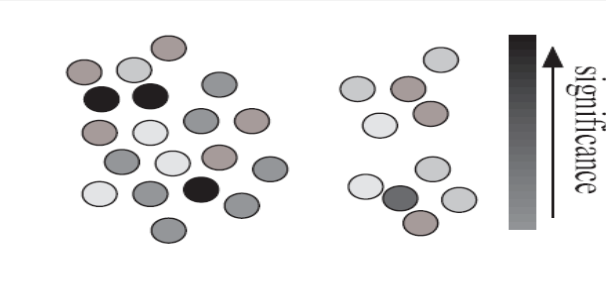
\includegraphics[width=0.32\linewidth, height=0.2\linewidth]{desired_patterns_1.png}
  \label{fig:desired1}}
\quad
\subfigure[redundancy-aware top-k]{%
  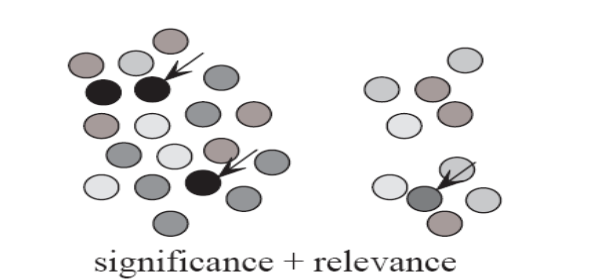
\includegraphics[width=0.32\linewidth, height=0.2\linewidth]{desired_patterns_2.png}
  \label{fig:desired2}}
\subfigure[traditional top-k]{%
  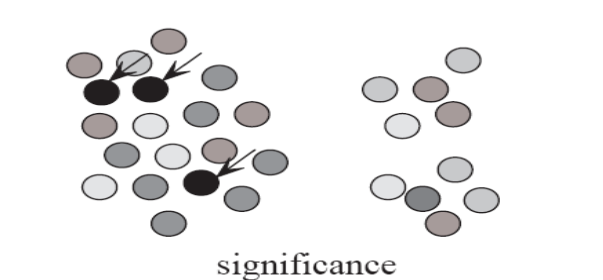
\includegraphics[width=0.32\linewidth, height=0.2\linewidth]{desired_patterns_3.png}
  \label{fig:desired3}}
\quad
\subfigure[summarization]{%
  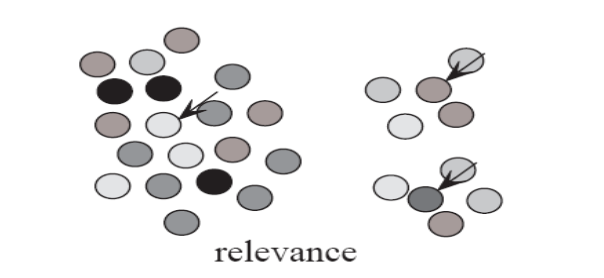
\includegraphics[width=0.32\linewidth, height=0.2\linewidth]{desired_patterns_4.png}
  \label{fig:desired4}}
%
\caption{Desired patterns: high significance \& low redundancy}
\label{fig:desired}
\end{figure}

Use \textbf{MMS (Maximal Marginal Significance)} for measuring the combined significance of a pattern set.\footnote{Xin et al., Extracting Redundancy-Aware Top-K Patterns, KDD’06.}

%--
\subsection{Mining Colossal Patterns}
\subsubsection{Pattern-Fusion}
\textbf{Pattern fusion strategy:} fuse small patterns together in one step to generate new pattern candidates of significant sizes.\\

Subpatterns $\alpha_1$ to $\alpha_k$ cluster tightly around the colossal pattern $\alpha$ by sharing a similar support. Such subpatterns are \textbf{core patterns} of $\alpha$. A colossal pattern can be generated by merging a set of core patterns.

\subsubsection{Robustness of Colossal Patterns}
\begin{definition}
For a frequent pattern $\alpha$, a subpattern $\beta$ is a $\mathbf{\tau}$\textbf{-core pattern} of $\alpha$ if $\beta$ shares a similar support set with $\alpha$, i.e., 
\begin{equation*}
\frac{\abs{D_\alpha}}{\abs{D_\beta}} \geqslant \tau, 0 < \tau \leqslant 1, 
\end{equation*}
where $\tau$ is called the \textbf{core ratio}.
\end{definition}

\begin{definition}
\textbf{$\mathbf{(d, \tau)}$-robustness}\footnote{Robustness - прочность}: a pattern $\alpha$ is $(d, \tau)$-robust if d is the maximum number of items that can be removed from $\alpha$ for the resulting pattern to remain a $\tau$-core pattern of $\alpha$:
\begin{equation*}
d = \max_{\beta}\{\abs{\alpha} - \abs{\beta} \mid \beta \subseteq \alpha\text{, and }\beta\text{ is a }\tau\text{-core pattern of }\alpha\}
\end{equation*}
\end{definition}

For a pattern $\alpha$ let $C_\alpha$ be the set of all its core patterns for a specified $\tau$:
\begin{equation*}
C_\alpha = \{\beta \mid \beta \subseteq \alpha, \frac{\abs{D_\alpha}}{\abs{D_\beta}} \geqslant \tau\}
\end{equation*}

\begin{theorem}
For a $(d, \tau)$-robust pattern $\alpha$:
\begin{equation*}
\abs{C_\alpha} \geqslant 2^d
\end{equation*}
\end{theorem}

\textbf{Robustness of Colossal Patterns}: a colossal pattern tends to have
much more core patterns than small patterns. Such core patterns can be clustered together to form <<dense balls>> based on pattern distance defined by 
\begin{equation*}
Dist(\alpha, \beta)=1-\frac{\abs{D_\alpha \cap D_\beta}}{\abs{D_\alpha \cup D_\beta}}
\end{equation*}

\begin{theorem}
For two patterns $\beta_1, \beta_2 \in C_\alpha$ 
\begin{equation*}
Dist(\beta_1, \beta_2) \leqslant r(\tau)\text{, where }r(\tau)=1-\frac{1}{2/\tau-1}
\end{equation*}
\end{theorem}

\subsubsection{The Pattern-Fusion Algorithm}
\begin{itemize}
\item Initialization (Creating initial pool): Use an existing algorithm to mine all frequent patterns up to a small size, e.g., 3
\item Iteration (Iterative Pattern Fusion):
\begin{itemize}
\item At each iteration, K seed patterns are randomly picked from the current pattern
pool
\item For each seed pattern thus picked, we find all the patterns within a bounding ball centered at the seed pattern
\item All these patterns found are fused together to generate a set of super-patterns
\item All the super-patterns thus generated form a new pool for the next iteration
\end{itemize}
\item Termination: when the current pool contains no more than K patterns at the beginning of an iteration
\end{itemize}

%--
\subsection{Recommended Readings}
\begin{itemize}
\item R. Srikant and R. Agrawal, <<Mining generalized association rules>>, VLDB'95
\item Y. Aumann and Y. Lindell, <<A Statistical Theory for Quantitative Association Rules>>, KDD'99
\item D. Xin, J. Han, X. Yan and H. Cheng, <<On Compressing Frequent Patterns>>, Knowledge and Data Engineering, 60(1): 5-29, 2007
\item D. Xin, H. Cheng, X. Yan, and J. Han, <<Extracting Redundancy-Aware Top-K Patterns>>, KDD'06
\item F. Zhu, X. Yan, J. Han, P. S. Yu, and H. Cheng, <<Mining Colossal Frequent Patterns by Core Pattern Fusion>>, ICDE'07
\item J. Han, H. Cheng, D. Xin, and X. Yan, <<Frequent Pattern Mining: Current Status and Future Directions>>, Data Mining and Knowledge Discovery, 15(1): 55-86, 2007
\end{itemize}